\newif\ifpdf
\ifx\pdfoutput\undefined
\pdffalse % we are not running PDFlatex
\else
\pdfoutput = 1 % we are running PDFlatex
\pdftrue
\fi

%% ****** Start of file template.aps ****** %
%%
%%
%%   This file is part of the APS files in the REVTeX 4 distribution.
%%   Version 4.0 of REVTeX, August 2001
%%
%%
%%   Copyright (c) 2001 The American Physical Society.
%%
%%   See the REVTeX 4 README file for restrictions and more information.
%%
%
% This is a template for producing manuscripts for use with REVTEX 4.0
% Copy this file to another name and then work on that file.
% That way, you always have this original template file to use.
%
% Group addresses by affiliation; use superscriptaddress for long
% author lists, or if there are many overlapping affiliations.
% For Phys. Rev. appearance, change preprint to twocolumn.
% Choose pra, prb, prc, prd, pre, prl, prstab, or rmp for journal
%  Add 'draft' option to mark overfull boxes with black boxes
%  Add 'showpacs' option to make PACS codes appear
%  Add 'showkeys' option to make keywords appear

%\documentclass[aps,prl,preprint,superscriptaddress]{revtex4}
%\documentclass[aps,prl,twocolumn,groupedaddress]{revtex4}

\documentclass [11pt, a4paper, openany, twoside=off] {article}
%\documentclass [landscape, 11pt, a4paper, openright, oneside] {article}
%\documentclass[aps,prl,preprint,groupedaddress]{revtex4}

\usepackage {amsmath, amssymb, amsfonts}
\usepackage {graphics}
\usepackage {graphicx}
\usepackage {longtable}
\usepackage {pgf,tikz,url}
\usepackage {float,afterpage} % for putting figure exactly where you want to, see appendix here
\usepackage {verbatim} % for begin comment, end comment
\usetikzlibrary{arrows,automata,shapes,snakes,backgrounds,topaths,petri}
%\usepackage {subfigure}
\usepackage{chemarr} % for xrightleftharpoons
\usepackage{lscape}
\usepackage{setspace}
\usepackage{subfig}

\newcommand{\ie}{{\em i.e. }}
\newcommand{\eg}{{\em e.g. }}
\newcommand{\cf}{{\em c.f. }}
\newcommand{\etc}{{\em etc. }}

\oddsidemargin 0.1in
%\evensidemargin 0.1in
\textwidth 6.1in 



% You should use BibTeX and apsrev.bst for references
% Choosing a journal automatically selects the correct APS
% BibTeX style file (bst file), so only uncomment the line
% below if necessary.
%\bibliographystyle{apsrev}
%\bibliographystyle{unsrt}
%\bibliographystyle{ieeetr}
%\bibliographystyle{interface}

\usepackage[sort&compress]{natbib}
\bibpunct{(}{)}{;}{a}{}{}
\setcounter{tocdepth}{2}
\setcounter{secnumdepth}{2}

\bibliographystyle{emborep2}

%\onehalfspacing
%\doublespacing

\title{ \emph{cuda-sim} \\ GPU accelerated biochemical network simulation}
\author{{\bf Yanxiang Zhou and Chris Barnes} }

\begin{document}
\maketitle

\newpage\tableofcontents\newpage

\section{Overview}
Graphics processing units (GPUs) have a highly parallel architecture with a high percentage of silicon dedicated to arithmetic operations and thus are suited to computationally intensive applications that can be parallelized. Biochemical network simulation is one such example as often analysis of models requires hundreds and thousands of simulations in order to understand parameter spaces, calculate probability distributions or perform simulation based inference.
\\
\\
There are a number of manufacturers providing programmable GPUs. NVIDIA has developed a hardware/software architecture called Compute Unified Device Architecture (CUDA) that has received considerable interest from the scientific community because it provides a C API that can be used for general purpose computation. {\it cuda-sim} uses PyCUDA which is a Python wrapper around CUDA and provides a flexible interface to the GPU.
\\
\\
In CUDA, small codes that run on the GPU are called {\it kernels}. A single kernel is run by multiple threads arranged into a thread block. Blocks in turn are arranged into a grid. Grids and blocks can be one, two or three dimensional. Since the GPU executes the same code on different data this type of architecture is known as Single Instruction Multiple Data (SIMD). Normal CPU clusters perform Multiple Instruction Multiple Data (MIMD) and this difference in computing paradigm can make porting of existing code to the GPU time consuming with only certain applications being suitable. To complicate things further, the GPU has different memory types, each with different properties such as access speeds and caching.
\\
\\
To run the tools in {\it cuda-sim}, no in-depth knowledge of CUDA and GPU computing is needed. Despite this there are some things to be aware of.
\subsection{Runtime limit on kernels}
All operating systems have watchdog timers that monitor the graphics output to detect if the GPU has frozen. As a consequence, the watchdog timer is supposed to terminate kernel calls if they run for more than 5 seconds. For this reason, we recommend running computationally intensive simulations on a separate graphics card that is not connected to a monitor. This issue can be circumvented on Linux by running with the X server disabled. To do this you can issue the command \verb$ sudo /sbin/init 3$ to kill the X server. 

\subsection{Lsoda requires double precision support}
Most older cards only support floating point arithmetic but ODE integration using LSODA requires CUDA GPUs that support double precision. Only cards that have compute capability 1.3 and greater support double precision. You can see what compute capability your cards support by looking in the NVIDA CUDA programming guide (Appendix A) or on the CUDA website.

\newpage
\section{Installation}
More detailed installation instructions can be found in the \verb$README.txt$ that accompanies the package.

\subsection{Prerequisites}
{\it cuda-sim} requires the following packages to be first installed
\begin{itemize}
\item \textbf{CUDA toolkit}
\item \textbf{numpy}
\item \textbf{pycuda}
\item \textbf{libsbml} (only for SBML parsing)
\end{itemize}

\subsection{Linux/Mac OS X installation instructions}
Once all required dependencies have been installed successfully and {\em cuda-sim} downloaded, installing just requires the following
\begin{verbatim}
$ tar xzf cuda-sim-VERSION.tar.gz
$ cd cuda-sim-VERSION
$ sudo python setup.py install 
\end{verbatim}
To install to a custom directory, the last line should be replaced with
\begin{verbatim}
$ sudo python setup.py install --prefix=<dir>
\end{verbatim}
which will place the package into the directory
\begin{verbatim}
<dir>/lib/python2.X/site-packages/
\end{verbatim}
where X is the python version.
     
        

\newpage
\section{Quick tutorial}
The following tutorial describes the essential steps for running \emph{cuda-sim} using a SBML model with custom parameters. For testing the software package with ready-to-run scripts see section Examples.\\ 

\begin{enumerate}
    \item Create a new folder.
    \item Create a text file for parameters and initialization values respectively in this folder. Separate parameters and species with white-spaces and each set of parameters and species with a linebreak (for examples see \verb$parameter.dat$ and \verb$species.dat$ files in \verb$example/ex01_immdeath/$ or \verb$example/ex02_p53/$). 
    \item Copy \verb$runExample.py$ (can be found in \verb$example/$) to the previously created folder.
    \item Open \verb$runExample.py$ in your folder with a text editor.
    \item Specify the location of your SBML model file in the line \verb$xmlModel = ""$.\\ (E.g. set \verb$xmlModel="/home/myFolder/myModel.xml"$)
    \item Specify the location of your parameter and initialization file in the lines\\ \verb$parameterFile = ""$ and \verb$speciesFile = ""$.\\ (E.g. set \verb$parameterFile = "param.dat"$ and \verb$speciesFile = "species.dat"$). 
    \item Decide which type of simulation you want to use by setting the line \\\verb$integrationType = "SDE"$ to the simulation type. \\(I.e. \verb$integrationType = "ODE"$ for ODE integration or\\ \verb$integrationType = "MJP"$ for using the Gillespie algorithm).
    \item Leave everything else as is, save and close \verb$runExample.py$.
    \item Run \verb$runExample.py$ (by typing \verb$python runExample.py$ in the console).
    \item The simulation results can be found in the newly created folder \verb$results/$.
\end{enumerate}

%\subsection{Troubleshooting}


\subsection{Troubleshooting}
If any problems with the package occur, please provide the SBML model, the edited \verb$runExample.py$ script, the parameter and initialization file, the error message and as many specifications of the running system as possible (e.g. Python version, PyCUDA version, OS, GPU specifications) and contact us!

\newpage
\section{Examples}
Two examples are provided in the \verb$examples$ folder that accompanies the package.

\subsection{Example1 : Immigration death}
This example models a simple immigration-death process. The model contains one species, has two reactions and is encoded in the SBML file \verb$immigration-death.xml$.
To run this example do the following:
\begin{verbatim}
$ cd examples/ex01_immdeath 
$ python runImmdeath.py
\end{verbatim}
This script reads in the files \verb$param.dat$ and \verb$species.dat$ which contain the parameters and initial conditions respectively (for the example 1000 sets of parameters and initial conditions were generated); each line represents the value for an individual thread. The simulation results are written into \verb$results/immdeath_result.txt$. 

If \verb$R$ has been installed the results can be plotted using the \verb$plot.R$ script by running R and executing the script in R (Figure~\ref{fig:ex_immdeath}):
\begin{verbatim}
$ source('plot.R')
\end{verbatim}
\begin{figure}[h!]%figure1
	\centering
	\subfloat[]{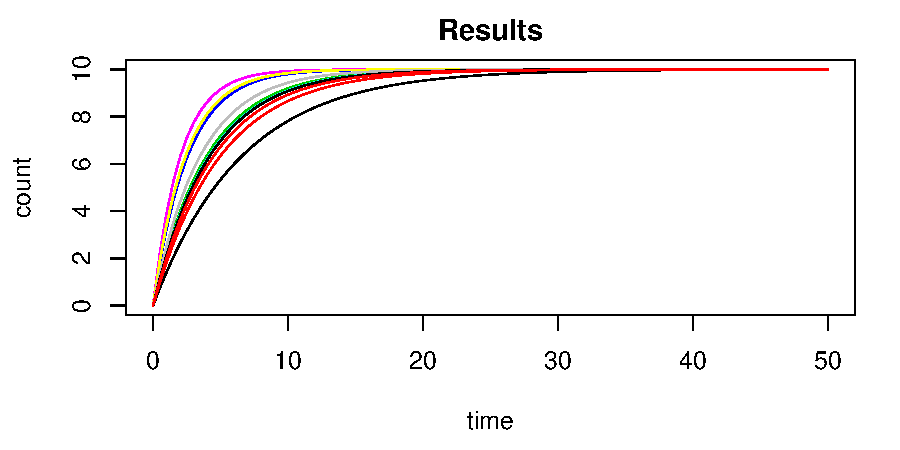
\includegraphics[width=0.45\textwidth]{figures/immdeath_ode.pdf}}
	\subfloat[]{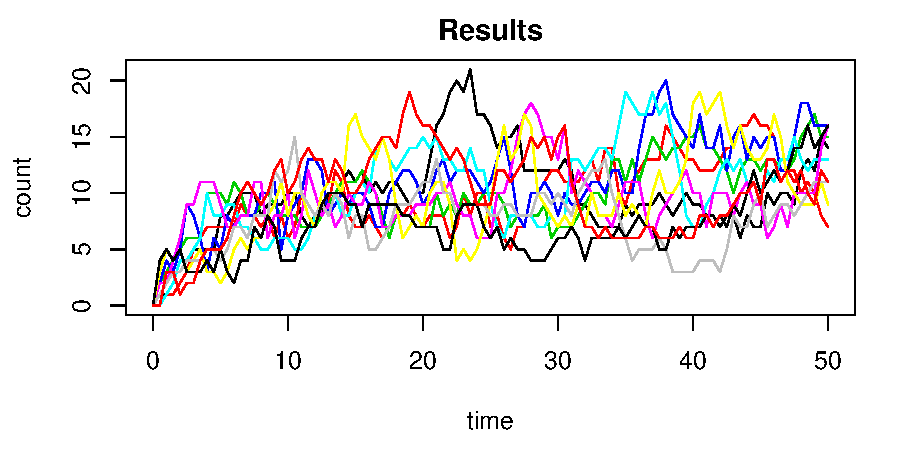
\includegraphics[width=0.45\textwidth]{figures/immdeath_mjp.pdf}}
	\caption{Simulation results obtained for the immigration-death process for (a) ODEs and (b) MJPs as described above.}
	\label{fig:ex_immdeath}
\end{figure}

\newpage
\subsection{Example2 : p53-Mdm2 oscillations}
This example models the p53-Mdm2 negative feedback loop \citep{??}. The model contains three species, has two reactions and is encoded in the SBML file \verb$p53model.xml$.
To run this example do the following
\begin{verbatim}
$ cd examples/ex02_p53
$ python runp53.py
\end{verbatim}
This script reads in the files \verb$param.dat$ and \verb$species.dat$ which contain the parameters and initial conditions respectively (for the example 1000 sets of parameters and initial conditions were generated); each line represents the value for an individual thread. The simulation results are written into \verb$results/p53_result.txt$.

%To change the simulation type, open \verb$runp53.py$ in a text editor and change the following line from\\
%\verb$integrationType = "ODE"$ to \verb$#integrationType = "ODE"$ and\\
%Then chamge one of the other lines (for example for the SDE) from\\
%\verb$#integrationType = "SDE"$ to \verb$integrationType = "SDE"$
If \verb$R$ has been installed the results can be plotted using the \verb$plot.R$ script by running R and executing the script in R (Figure~\ref{fig:ex_p53}):
\begin{verbatim}
$ source('plot.R')
\end{verbatim}

\begin{figure}[h!]%figure1
	\centering
	\subfloat[]{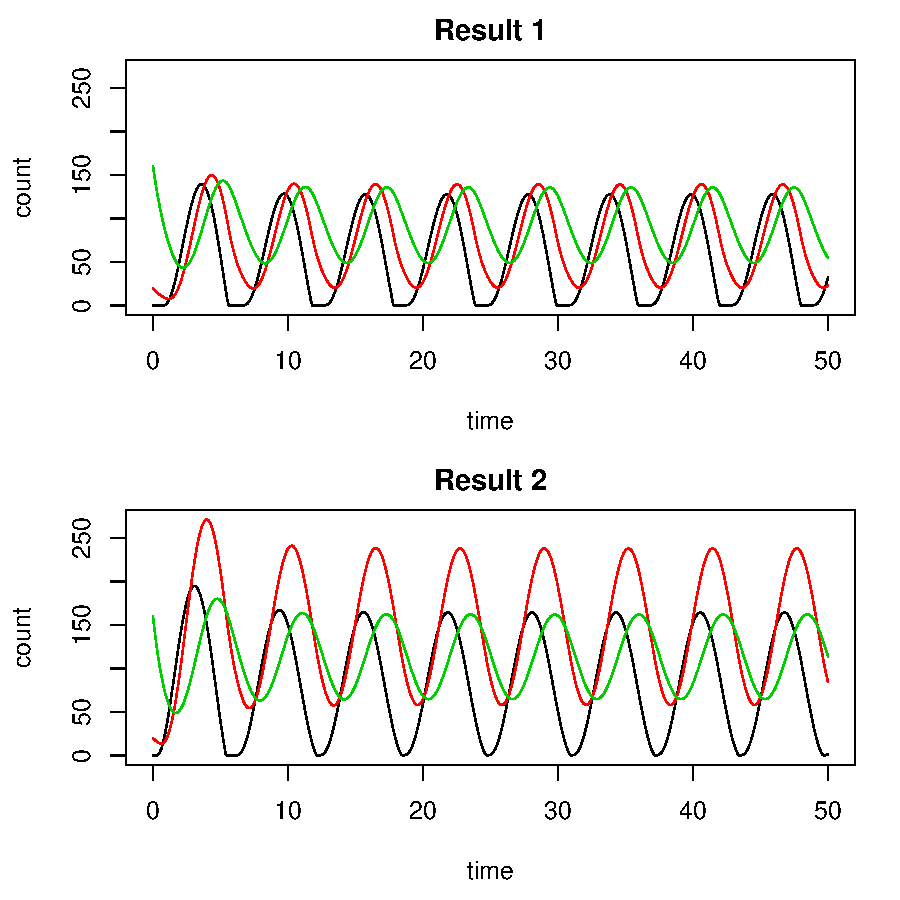
\includegraphics[width=0.45\textwidth]{figures/p53_ode.pdf}}
	\subfloat[]{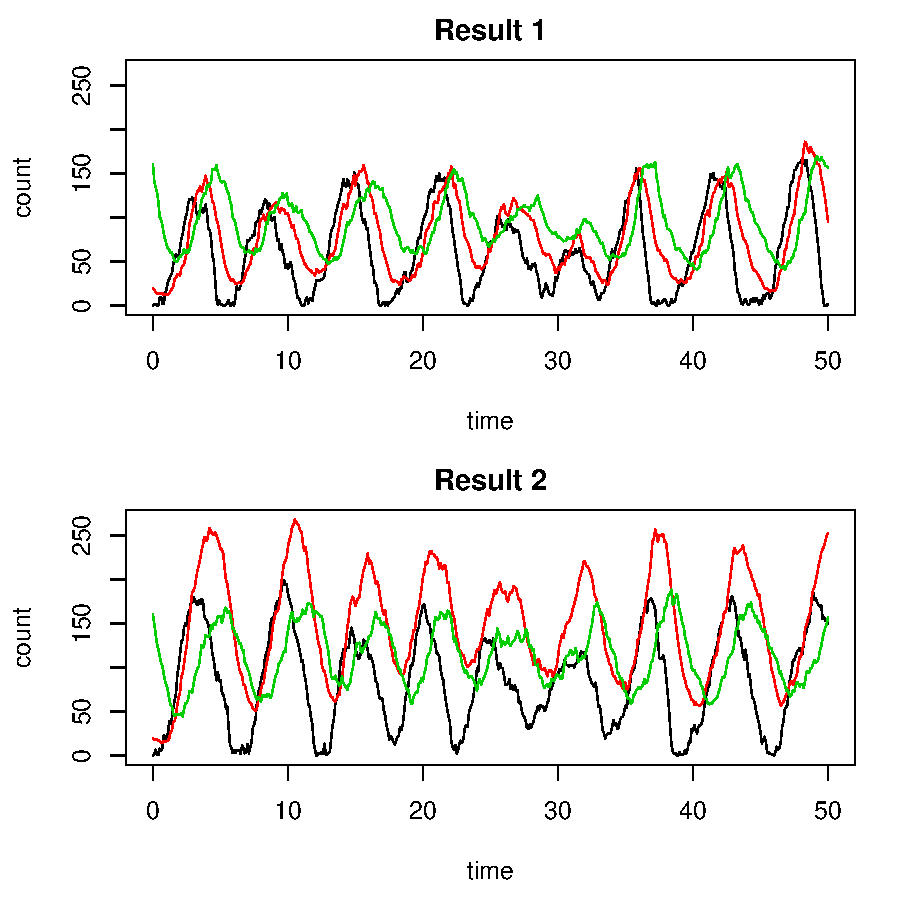
\includegraphics[width=0.45\textwidth]{figures/p53_sde.pdf}}
	\caption{Simulation results obtained for the p53-Mdm2 negative feedback loop for (a) ODEs and (b) SDEs as described above.}
	\label{fig:ex_p53}
\end{figure}

\newpage
\section{Functionality}
\subsection{SBMLParser.py}
The SBML parser provides the ability to generate CUDA kernels for ODE, SDE and MJP simulations using the pre-implemented algorithms. The SBML parser is derived from the SBML parser for the ABC-SysBio package. %\citep{??, ??}.
\subsubsection{Call SBMLParser}
To access the SBMLParser the following function needs to be called (multiple models can be parsed at once):
\begin{center}
\texttt{importSBMLCUDA([xmlModel],[integrationType],[modelName],outpath=temp)}
\end{center}
\begin{itemize}
	\item \textbf{{[}xmlModel{]}} Array of strings with the location of the SBML files.
	\item \textbf{{[}integrationType{]}} Array of strings with the simulation types to be used (i.e. ``ODE", ``SDE" or ``MJP").
	\item \textbf{{[}modelName{]}} Array of strings with the names of the models.
	\item \textbf{outpath} String specifying the folder where the CUDA kernels should be saved.
\end{itemize}


\subsection{Simulator.py}
The Simulator class is the superclass for the Lsoda, EulerMaruyama and Gillespie classes. Here, all functions that the user should be able to access are defined. Furthermore, all parameters regulating GPU calls (like blocksize and gridsize) are defined in \verb$Simulator.py$. %For further details regarding the design principles of this superclass see the section Extend the package.

\subsection{Lsoda.py}
The Lsoda class uses the LSODA algorithm to solve ODEs. 

\subsubsection{Instantiating Lsoda}
To run the ODE solver, firstly, the CUDA code has to be compiled. This is done by instantiating:
\begin{center}
\texttt{Lsoda(timepoints, cudaCode)}
\end{center}
\begin{itemize}
	\item \textbf{timepoints} Array of floats specifying the time points at which the integration results should be printed out. Time points do not need to be equidistant.
	\item \textbf{dt} Float specifying time step distances (no relevance for ODE integration)
	\item \textbf{cudaCode} String specifying CUDA kernel.
\end{itemize}

\subsubsection{Run ODE integration}
To run the ODE integration the following function has to be called:
\begin{center}
\texttt{run(parameters, initValues, timing=boolean)}
\end{center}
\begin{itemize}
	\item \textbf{parameters} Array of arrays of floats specifying parameters for every thread and all different parameters in the model. The length of the parameters array defines the total number of threads and should be equal to the length of the initValues array.
	\item \textbf{initValues}  Array of arrays of floats specifying initialization values for every thread and all different species in the model. The length of the initialization values array should be equal to the length of the parameters array.
\item \textbf{timing} Boolean specifying if the runtime should be reported.
\end{itemize}

\subsubsection{Returned result}
The \verb$run$ function returns the result as four-dimensional array containing float values in the follwing form (this is the same as for EulerMaruyama and Gillespie):
\begin{center}
\texttt{[\#threads][beta][\#timepoints][speciesNumber]}
\end{center}
\begin{itemize}
	\item \textbf{\#threads} Index for different threads.
	\item \textbf{beta} Index for different repeats with the same set of parameters. (Can only be 0 since no repeats for ODE integrations will be carried out using the same set of parameters).
	\item \textbf{\#timepoints} Index for each time point that was specified when calling \verb$run$.
	\item \textbf{speciesNumber} Index for different species.
\end{itemize}


\subsection{EulerMaruyama.py}
The EulerMaruyama class uses the Euler-Maruyama algorithm to simulate SDEs. 
\subsubsection{Instantiating EulerMaruyama}
To run SDE simulations, firstly, the CUDA code has to be compiled. This is done by instantiating:
\begin{center}
\texttt{EulerMaruyama.EulerMaruyama(timepoints, cudaCode, dt, beta)}
\end{center}
\begin{itemize}
\item \textbf{timepoints} Array of floats specifying the time points at which the integration results should be printed out. Timepoints do not need to be equidistant.
\item \textbf{cudaCode} String specifying CUDA kernel.
\item \textbf{dt} Float specifying time step distances.
\item \textbf{beta} Integer specifying the number of repeated simulations with the same set of parameters. Should be used to explore sensitivity of the results to noise.
\end{itemize}

\subsubsection{Run SDE simulation}
To run the simulation, following function has to be called (this is the same as for Gillespie):
\begin{center}
\texttt{run(parameters, initValues, timing=boolean, seed=seedValue)}
\end{center}
\begin{itemize}
	\item \textbf{parameters} Array of arrays of floats specifying parameters for every thread and all different parameters in the model. The length of the parameters array defines the total number of threads and should be equal to the length of the initValues array.
	\item \textbf{initValues}  Array of arrays of floats specifying initialization values for every thread and all different species in the model. The length of the initialization values array should be equal to the length of the parameters array.
	\item \textbf{timing} Boolean specifying if the runtime should be reported.
	\item \textbf{seed} Integer between 0 and 4294967295 to seed random number generators. For consecutive runs, the optional seed can be left out since it will be updated internally.
\end{itemize}

\subsubsection{Returned result}
The \verb$run$ function returns the result as four-dimensional array containing float values in the follwing form (this is the same as for Lsoda and Gillespie):
\begin{center}
\texttt{[\#threads][beta][\#timepoints][speciesNumber]}
\end{center}
\begin{itemize}
	\item \textbf{\#threads} Index for different threads.
	\item \textbf{beta} Index for different repeats with the same set of parameters.
	\item \textbf{\#timepoints} Index for each time point that was specified when calling \verb$run$.
	\item \textbf{speciesNumber} Index for different species.
\end{itemize}


\subsection{Gillespie.py}
The Gillespie class uses the Gillespie algorithm to simulate MJPs. 
\subsubsection{Instantiating Gillespie}
To run MJP simulations, firstly, the CUDA code has to be compiled. This is done by instantiating:
\begin{center}
\texttt{Gillespie(timepoints, cudaCode, beta)}
\end{center}
\begin{itemize}
	\item \textbf{timepoints} Array of floats specifying the time points at which the integration results should be printed out. Time points do not need to be equidistant.
	\item \textbf{cudaCode} String specifying CUDA kernel.
	\item \textbf{beta} Integer specifying the number of repeated simulations with the same set of parameters. Should be used to explore sensitivity of the results to noise.
\end{itemize}

\subsubsection{Run MJP simulation}
To run the simulation following function has to be called (this is the same as for EulerMaruyama):
\begin{center}
\texttt{run(parameters, initValues, timing=boolean, seed=seedValue)}
\end{center}
\begin{itemize}
	\item \textbf{parameters} Array of arrays of floats specifying parameters for every thread and all different parameters in the model. The length of the parameters array defines the total number of threads and should be equal to the length of the initValues array.
	\item \textbf{initValues}  Array of arrays of floats specifying initialization values for every thread and all different species in the model. The length of the initialization values array should be equal to the length of the parameters array.
	\item \textbf{timing} Boolean specifying if the runtime should be reported.
	\item \textbf{seed} Integer between 0 and 4294967295 to seed random number generators. For consecutive runs the optional seed can be left out since it will be updated internally.
\end{itemize}

\subsubsection{Returned result}
The \verb$run$ function returns the result as four-dimensional array containing float values in the follwing form (this is the same as for Lsoda and EulerMaruyama):
\begin{center}
\texttt{[\#threads][beta][\#timepoints][speciesNumber]}
\end{center}
\begin{itemize}
	\item \textbf{\#threads} Index for different threads.
	\item \textbf{beta} Index for different repeats with the same set of parameters.
	\item \textbf{\#timepoints} Index for each time point that was specified when calling \verb$run$.
	\item \textbf{speciesNumber} Index for different species.
\end{itemize}

\newpage
\section{Providing custom CUDA kernels}
Instead of using the SBML parser, it is also possible to directly provide CUDA kernels. In the following sections, the most important aspects of the CUDA kernels for the different algorithms are described.
\subsection{General}
\subsubsection{Header}
Firstly, all CUDA kernels need to specify the number of species, parameters and reactions. This is done using \verb$define$ statements (please note that there is one additional parameter for the compartment):
\begin{verbatim}
#define NSPECIES 3
#define NPARAM 9
#define NREACT 6
\end{verbatim}

\subsubsection{Parameters}
For all three algorithms, parameters are stored in texture memory. The parameters can be accessed by calling the following function:
\begin{verbatim}
tex2D(param_tex,index,tid)
\end{verbatim}
The argument \verb$index$ has to be replaced by the index of the parameter to access. The index 0 is always reserved for the compartment parameter. Since texture memory is read-only memory, parameters cannot be modified directly. Rather a wrapping function has to be defined, that, depended on the time or other parameters, returns a modified parameter. E.g. if you want the parameter with index 3 to be doubled between the time points 10 and 15 you have to define the following function:
\begin{verbatim}
__device__ float function(float a1, float t){
    if(t > 10 && t < 15)
        return 2*a1;
    else
        return a1;
}
\end{verbatim}
and instead of calling the reference to the texture directly, the call has to be wrapped with the function defined above:
\begin{verbatim}
function(tex2D(param_tex,3,tid), t)
\end{verbatim}

\subsubsection{Species}
Species are stored in registers that can also be written. They can be directly accessed and changed by referencing with the index of the species:
\begin{verbatim}
y[index]
\end{verbatim}

\subsection{ODEs}
\subsubsection{Overview}
For solving ODEs, either the difference quotient for each species or the full Jacobian should be specified inside structures. In our examples and by using the provided SBML parser, difference quotients are used.  For details how to specify the Jacobian please refer to the comments in the header of \verb$cuLsoda_all.cu$.

\subsubsection{Specify difference quotients}
The struct frame should look as follows:
\begin{verbatim}
struct myFex{
    __device__ void operator()(int *neq, double *t, double *y, double *ydot){
    }
};
\end{verbatim}
Inside the \verb$operator$ function, the difference quotient for the species should be defined by specifying \verb$ydot$ for each species, e.g.:
\begin{verbatim}
ydot[0] = tex2D(param_tex,1,tid) * y[0];
\end{verbatim}

\subsection{SDEs}
\subsubsection{Overview}
For the SDEs, two versions of the code should be written. One for using texture memory and one for using shared memory for storing parameters. The only difference between these versions is how parameters are accessed. Both version should be put into the same file. The version for using texture memory should begin with the following comment:
\begin{verbatim}
//Code for texture memory
\end{verbatim}
and the version for using shared memory should begin with:
\begin{verbatim}
//Code for shared memory
\end{verbatim}
To access parameters via their index in shared memory, use the following call:
\begin{verbatim}
parameter[index]
\end{verbatim}
In contrast to parameters stored in texture memory (as described above), parameters in shared memory can also be directly changed. I.e. the following statement is possible:
\begin{verbatim}
parameter[0] = 1.5;
\end{verbatim}

\subsubsection{Step-function}
The function that is called in every time step should have this form for the version for using texture memory:
\begin{verbatim}
__device__ void step(float *y, unsigned *rngRegs, int tid){
}
\end{verbatim}
and for using shared memory, additionally, a pointer to the shared memory, where the parameters are stored is needed:
\begin{verbatim}
__device__ void step(float *parameter, float *y, unsigned *rngRegs){
}
\end{verbatim}
The constant of each time step is stored in the global constant:
\begin{verbatim}
DT
\end{verbatim}

\subsubsection{Normally distributed random number}
To generate normally distributed random numbers with a mean of 0 and a variance of \verb$DT$, call the following function:
\begin{verbatim}
randNormal(rngRegs,WarpStandard_shmem,sqrt(DT));
\end{verbatim}
It is \textbf{very important} that all threads in a warp call this function at the \textbf{same time}. No calls of this function should occur after any intra-warp divergence. This can be ensured if no conditional statements like \verb$if$s are place inside the \verb$step()$ function before a call to \verb$randNormal()$ is made.

\subsection{MJPs}
\subsubsection{Overview}
For using MJPs, the stochiometry matrix and a hazards function have to be specified.

\subsubsection{Stochiometry matrix}
The stochiometry specifies the changes of species if a certain reaction occurs. The ``matrix" has one column for each species and one row for each reaction. E.g. for a model with two species (X and Y) and the three following reactions:
\begin{itemize}
    \item $\emptyset \rightarrow X$
    \item $X \rightarrow 2Y$
    \item $Y \rightarrow \emptyset$
\end{itemize}
the stochiometry matrix should be defined the following way (with X being the first and Y being the second species):
\begin{verbatim}
__constant__ int smatrix[]={
    1.0,  0.0,
   -1.0,  2,0,
    0.0, -1.0
};
\end{verbatim}

\subsubsection{Hazards function}
The hazards function specifies the probability of each reaction occurring. For the example above, the hazards function would be defined as follows:
\begin{verbatim}
__device__ void hazards(int *y, float *h, float t, int tid){
    h[0] = tex2D(param_tex,1,tid);
    h[1] = tex2D(param_tex,2,tid)*y[0];
    h[2] = tex2D(param_tex,3,tid)*y[1];
}
\end{verbatim}
Here, each reaction is determined by another parameter. (Note that the indices begin with 1, since the 0-th parameter represents the compartment).

%\subsection{Extend the package}

\newpage
\section{Performance}
\emph{cuda-sim} was developed to increase the performance of simulating biochemical networks. Even though in comparison to simulations on single CPUs substantial performance gains are attained, to get the best performance out of GPUs, dependent on the model, further fine tuning may be required. In the following sections we discuss some of these issues. For a general introduction to the concepts of GPU computing and CUDA please refer to the NVIDIA CUDA Programming Guide and Dr. Dobb's introduction on CUDA -- ``CUDA, Supercomputing for the Masses".

\subsection{Using shared memory}
By using PyCUDA we can employ \em{runtime code generation}. We make use of this for SDE simulations and \em{cuda-sim} automatically determines at runtime if the parameters fit in shared memory. By using the faster shared memory instead of texture memory we could decrease the runtime for the p53-Mdm2 model by 2.4\%. The decrease in runtime will strongly depend on the memory access intensity. 

\begin{figure}[h!]%figure1
	\centering
	\includegraphics[width=0.45\textwidth]{figures/summary.pdf}
	\caption{Timing comparisons between using texture memory and shared memory. Timing for different numbers of simulations of length 100~hours using the p53-Mdm2 model storing the parameters in texture memory and shared memory. The decrease in runtime for using shared memory is indicated above the bars. All timing results are the averages from three runs.}
	\label{fig:ex_p53}
\end{figure}

\subsection{Occupancy}
A major determinant of performance is how well latency is hidden by multiple warps per multiprocessor. In this case, warps that are not ready for execution can be ``parked" while other warps are executed. In general, it is therefore desirable to have a high number of warps per multiprocessor (occupancy). However, depending on the exact ratio of float point operations to memory access, there may be a value for occupancy above which no performance gain can be expected, because the multiprocessors are already working to their full capacity.

Since the maximum number of blocks per multiprocessor for all compute capabilities is restricted to 8, blocksizes of 96, 128 or 192 threads per block (or multiples thereof) for compute compatibility 1.0~\&~1.1, 1.2~\&~1.3 and 2.0 respectively are required to maximize occupancy. But this only holds true if the number of registers or shared memory used per kernel are not limiting the number of warps per multiprocessor. In our case, the number of registers will be the limiting factor for the maximum number of warps per multiprocessor. Therefore the blocksizes for achieving a high occupancy will not be those values mentioned above and vary between different models.

Another issue with choosing the blocksize is the number of unused threads depending on the total number of threads the user wants to run. In the worst case, a complete block (minus one thread) might be needed to be initialized and run (for example when a blocksize of 64 threads is chosen, and 65 threads should be run). The smaller the blocksize is, the smaller the wasted number of threads will be. This is especially important for running smaller numbers of threads.

For the reasons mentioned above, we set the default blocksize to 64 (or reduce it to 32, if the number of registers used per kernel only allows 32 threads per block). We think that 64 is a good compromise between having a high occupancy and a small overhead. For specific applications (especially when you are running very time-consuming simulations) you might want to test if other blocksizes will give you an improved performance.
%include test figure!

%We also fixed the maximum number of blocks that will be submitted to the GPU per run to 512. This is simply due to the reason that in our current implementation, the Mersenne Twister RNG for the Gillespie algorithm is limited to 32,768 threads. As for the blocksize, for specific applications you might want to change this limit.

%\subsection{On-chip memory}

%\subsection{Gillespie algorithm and warp divergence}



\end{document}
%
% ****** End of file template.aps ******
